\chapter{Implementacija i korisničko sučelje}
		
		
		\section{Korištene tehnologije i alati}
		
			
			 
			 Za timsku komunikaciju koristili smo WhatsApp\footnote{https://www.whatsapp.com/} koji nam je pružio brz i jednostavan medij. Za vizualizaciju i modeliranje sustava, Astah Professional\footnote{http://astah.net/editions/professional} bio je naš odabir, omogućio nam je izradu UML dijagrama koji su olakšali razumijevanje strukture i funkcionalnosti projekta.\\
			 
			 Git\footnote{https://git-scm.com/} je bio ključan u procesu upravljanja izvornim kodom, omogućavajući nam upravljanje inačicama i suradnju na projektu. Udruženi repozitorij projekta smješten na GitHub\footnote{https://github.com} platformi pružio je centralizirano mjesto za pohranu, pregled i praćenje promjena u kodu.\\
			 
			 Za razvoj softvera koristili smo Rider\footnote{https://www.jetbrains.com/rider/} integrirano razvojno okruženje (IDE) koje nam je omogućilo učinkovitiju izradu aplikacije.\\
			 
			 Na strani backenda, odabrali smo ASP.NET Core radni okvir\footnote{https://dotnet.microsoft.com/en-us/apps/aspnet/} u kombinaciji s jezikom C\#\footnote{https://docs.microsoft.com/en-us/dotnet/csharp/}, a za frontend smo se uz standardni HTML,\footnote{https://www.w3.org/html/} CSS\footnote{https://www.w3.org/Style/CSS/Overview.en.html} i JS\footnote{https://www.javascript.com/} oslonili na htmx\footnote{https://htmx.org/} radi njegove jednostavnosti.\\
			 
			 Baza podataka implementirana u PostgreSQL-u\footnote{https://www.postgresql.org/} smještena je na poslužitelju u oblaku Microsoft Azure\footnote{https://portal.azure.com/}.\newline
			
			
			\eject 
		
	
		\section{Ispitivanje programskog rješenja}
		
			Opsežno ispitivanje nažalost nismo napravili, no testirali smo programsko rješenje ručno.
			
			
			\eject 
		
		
		\section{Dijagram razmještaja}
			
			Dijagram razmještaja prikazuje topologiju sklopovlja i njegove programske potpore koji služe za implementaciju sustava u njegovom radnom okruženju. Na poslužiteljskom računalu se nalaze web poslužitelj i poslužitelj baze podataka. Korisnik se mora služiti web preglednikom da može pristupiti web aplikaciji. Sustav je baziran na arhitekturi "klijent - poslužitelj". Komunikacija između računala korisnika i poslužitelja se uspostavlja pomoću HTTP veze
			 \begin{figure}[hbt!]
			 	\centering
			 	\includegraphics[width = \textwidth]{slike/Dijagram razmještaja}
			 	\caption{Dijagram razmještaja}
			 	\label{fig:razmjestaj}
			 \end{figure}
			
			\eject 
		
			\section{Upute za puštanje u pogon}
				\label{sec:deployment}

				\textbf{Kreiranje Azure Računa}
				\begin{enumerate}
					\item Posjetite Azure portal i odaberite opciju za kreiranje novog računa.
					\item Slijedite korake registracije, uključujući verifikaciju identiteta i odabir pretplate.
				\end{enumerate}

				\textbf{Instalacija Visual Studio Code}
				\begin{itemize}
					\item Preuzmite i instalirajte Visual Studio Code (VSC) sa službene stranice: \url{https://code.visualstudio.com/}
				\end{itemize}

				\textbf{Instalacija Azure Tools Ekstenzije za VSC}
				\begin{itemize}
					\item U VSC, otvorite Extensions view (Ctrl+Shift+X) i pretražite "Azure Tools". Instalirajte ekstenziju koja će vam omogućiti upravljanje Azure resursima izravno iz VSC.
				\end{itemize}

				\textbf{Instalacija .NET 7.0 SDK}
				\begin{itemize}
					\item Preuzmite i instalirajte .NET 7.0 SDK kako biste mogli razvijati i testirati .NET aplikacije.
				\end{itemize}

				\textbf{Priprema Azure Resursa}
				\begin{enumerate}
					\item Stvaranje Azure Database za PostgreSQL:
					\begin{itemize}
						\item Prijavite se na Azure Portal.
						\item Odaberite "Create a resource" i potražite "Azure Database for PostgreSQL".
						\item Slijedite upute za stvaranje PostgreSQL instance, odabirom imena, konfiguracije performansi, te postavljanje administrator korisničkog imena i lozinke.
					\end{itemize}
					\item Stvaranje Azure App Service:
					\begin{itemize}
						\item Na Azure Portalu, odaberite "Create a resource" i potražite "Web App".
						\item Stvorite novu web aplikaciju, odaberite runtime okruženje koje odgovara vašoj .NET aplikaciji, i postavite potrebne parametre kao što su ime, plan cijena, i lokacija.
						\item Preporuke možete vidjeti na stranici: \url{https://learn.microsoft.com/en-us/azure/app-service/quickstart-dotnetcore?tabs=net70&pivots=development-environment-vscode}
					\end{itemize}
				\end{enumerate}

				\textbf{Deployment .NET Aplikacije na Azure}
				\begin{enumerate}
					\item Priprema Aplikacije za Deployment:
					\begin{itemize}
						\item Ukoliko ste instalirati Visual Studio Code, klikom na Terminal -> New Terminal stvorite terminal te upišite \texttt{git clone https://github.com/MarkoHaralovic/Nad} te odaberite gdje želite smjestiti klonirani git repozitorij.
						\item U istom terminalu upišite: \texttt{git checkout -b dev origin/dev} te se smjestite u direktorij \texttt{Nad\textbackslash izvorniKod\textbackslash StoZelisCitati\textbackslash StoZelisCitati} naredbom \texttt{cd Nad\textbackslash izvorniKod\textbackslash StoZelisCitati\textbackslash StoZelisCitati}
						\item U vašem razvojnom okruženju (VSC), koristite \texttt{dotnet publish} za kompilaciju i pripremu aplikacije. Navedite putanju do direktorija gdje će se stvoriti objavljena verzija, npr. \texttt{dotnet publish -c Release -o ./Publish}
					\end{itemize}
					\item Deployment korištenjem Azure CLI ili Visual Studio:
					\begin{itemize}
						\item Ako koristite Azure CLI, prijavite se na svoj Azure account koristeći \texttt{az login}.
						\item Nakon prijave, koristite sljedeću naredbu za deployment aplikacije: \texttt{az webapp up --name <app-name> --resource-group <resource-group-name> --location <location> --sku F1 --zip-file <path-to-zip>}
						\item Ako koristite Visual Studio, desni klik na projekt i odaberite "Publish". Slijedite upute za odabir cilja objave koji će biti Azure.
					\end{itemize}
				\end{enumerate}

				\begin{figure}[hbt!]
					\centering
					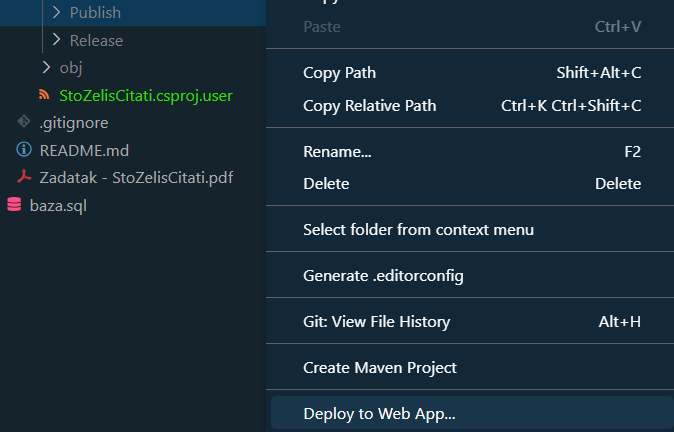
\includegraphics[width=\textwidth]{slike/deployment.png}
					\caption{Puštanje aplikacije u pogon preko Visual Studio Codea}
					\label{fig:vscode-deployment}
			   \end{figure}
			  

				\textbf{Konfiguracija Connection Stringa}
				\begin{enumerate}
					\item Postavljanje Connection Stringa:
					\begin{itemize}
						\item U Azure Portalu, idite na stranicu "App Service" vaše aplikacije.
						\item Pronađite odjeljak "Configuration" i dodajte novi connection string pod "Application settings".
						\item Format connection stringa trebao bi biti: \texttt{Server=<server-name>.postgres.database.azure.com;Database=<database-name>;Port=5432;User Id=<username>@<server-name>;Password=<password>;Ssl Mode=Require;}
					\end{itemize}
				\end{enumerate}

				\textbf{Praćenje Aplikacije}
				\begin{itemize}
					\item Konfigurirajte Azure Application Insights za praćenje performansi aplikacije i dijagnostiku problema.
				\end{itemize}

			